\documentclass[letterpaper, 11pt]{article}
\usepackage{amsmath}
\usepackage{float}
\usepackage{inputenc}
\usepackage[left=2cm, right=2cm, top=2cm, bottom=2cm]{geometry}
\usepackage{graphicx}
\usepackage{float}
\usepackage{caption}
\usepackage{extarrows}
\usepackage{xcolor}
\usepackage{lscape}
\usepackage{pdflscape}
\usepackage{pdfpages}
\usepackage{amssymb}

\usepackage{listings}
\usepackage{color}

%Default fixed font does not support bold face
\DeclareFixedFont{\ttb}{T1}{txtt}{bx}{n}{12} % for bold
\DeclareFixedFont{\ttm}{T1}{txtt}{m}{n}{12}  % for normal

% Custom colors
\definecolor{deepblue}{rgb}{0,0,0.5}
\definecolor{deepred}{rgb}{0.6,0,0}
\definecolor{deepgreen}{rgb}{0,0.5,0}


% color def
\definecolor{darkred}{rgb}{0.6,0.0,0.0}
\definecolor{darkgreen}{rgb}{0,0.50,0}
\definecolor{lightblue}{rgb}{0.0,0.42,0.91}
\definecolor{orange}{rgb}{0.99,0.48,0.13}
\definecolor{grass}{rgb}{0.18,0.80,0.18}
\definecolor{pink}{rgb}{0.97,0.15,0.45}

% listings
% Define a custom color
\definecolor{backcolour}{rgb}{0.95,0.95,0.92}
\definecolor{codegreen}{rgb}{0,0.6,0}

% Define a custom style
\lstdefinestyle{myStyle}{
    backgroundcolor=\color{backcolour},
    commentstyle=\color{codegreen},
    basicstyle=\ttfamily\footnotesize,
    breakatwhitespace=false,
    breaklines=true,
    keepspaces=true,
    numbers=left,
    numbersep=5pt,
    showspaces=false,
    showstringspaces=false,
    showtabs=false,
    tabsize=2,
    keywordstyle=\bfseries\color{blue},
}
\newcommand{\peq}{ \mathrel{+}= }
\newcommand{\muleq}{ \mathrel{*}= }

% Use \lstset to make myStyle the global default
\lstset{style=myStyle}

\title{Dynamic model of a Tilted-winged hexacopter}
\author{Sesha Charla}
\date{\today}


\begin{document}
\maketitle
\tableofcontents
\newpage

\section{Kinematics}

\begin{figure}[h]
    \begin{minipage}{0.49\textwidth}
        \begin{figure}[H]
            \centering
            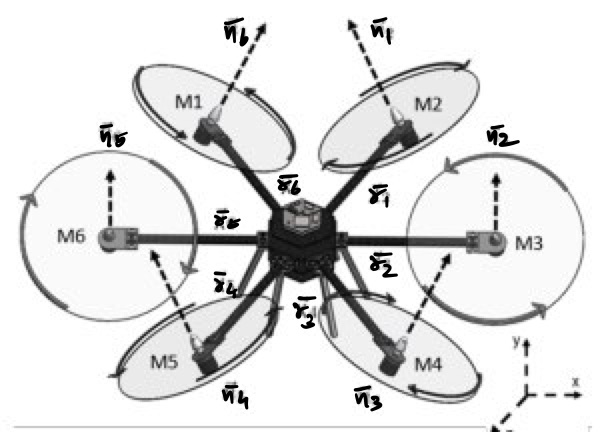
\includegraphics[width = 0.9\textwidth]{./figs/hex_copt-1.jpg}
        \end{figure}
    \end{minipage}
        \begin{minipage}{0.49\textwidth}
        \begin{figure}[H]
            \centering
            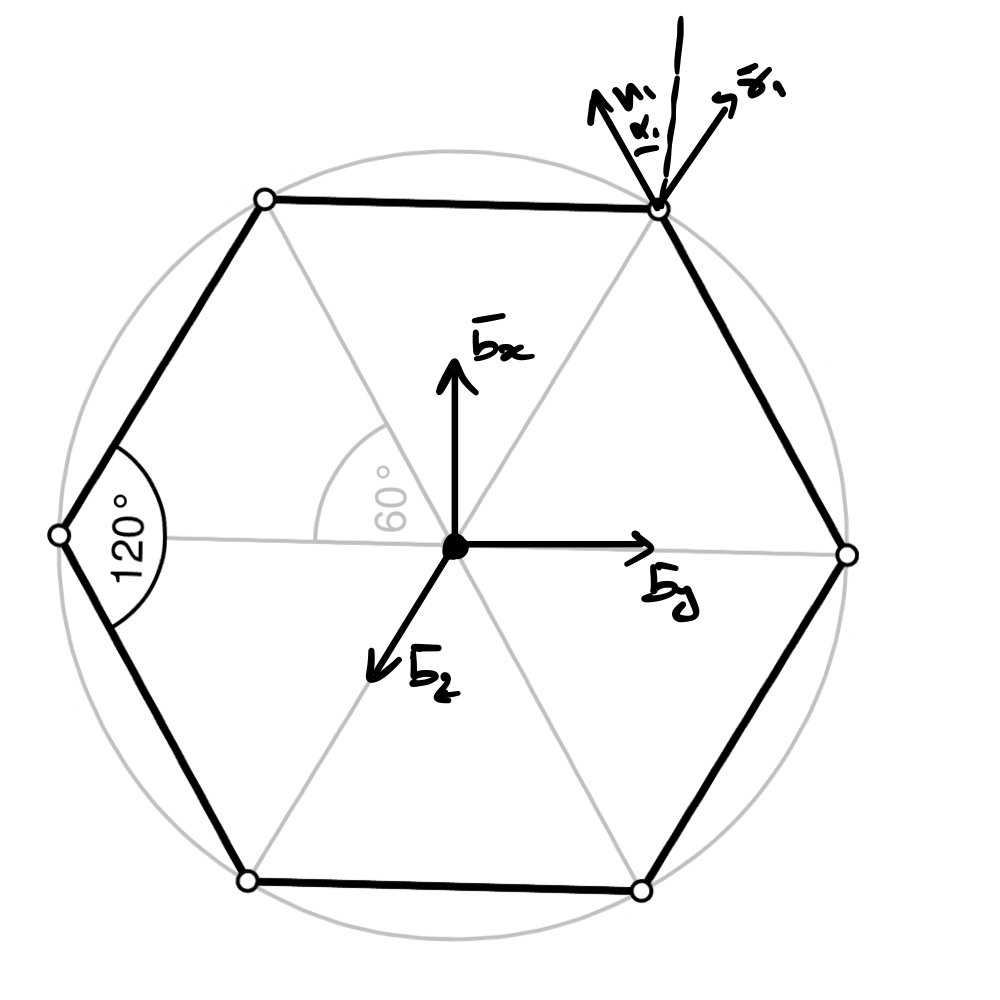
\includegraphics[width = 0.8\textwidth]{./figs/hex_copt-2.png}
        \end{figure}
    \end{minipage}
\end{figure}

\medskip

\subsection{Propeller angular velocity vectors}
Let, $b$ be the body-frame with $\{\pmb{b_x \, b_y \, b_z}\}$ as 3 mutually perpendicular right-handed unit vectors shuch that $\pmb{b_z}$ points downwards (in the direction of gravity), $\pmb{b}_x$ point forward and $\pmb{b}_y$ such that they form the right-handed system. let, $\pmb{n}_i$ be the unit vectors pointing 'upwards' perpendicular to the rotor-plane of $i^{th}$ propeller and $\pmb{r}_i$ be the radial vectors pointing outwards along the $i^{th}$ propeller shaft. the propeller tilt-angle $\alpha_i$ is conisdered positive along $\pmb{r}_i$, i.e., radially outwards.
\begin{align*}
   \therefore \alpha_i &= (-1)^{i} \alpha \qquad (\alpha_1 = -\alpha, \; \alpha_2 = \alpha \hdots) \\
   \implies \cos \alpha_i &= \cos \alpha  = c_{\alpha} \quad and\\
   \sin \alpha_i &= (-1)^{i} \sin \alpha = (-1)^{i} s_{\alpha}
\end{align*}

Let, $\gamma_i$ be the angle of the $i^{th}$ propeller shaft along $\pmb{b_z}$ (clockwise), i.e.,
\begin{align*}
\gamma_i &= \frac{i\pi}{3} - \frac{\pi}{6} = (2i-1)\frac{\pi}{6}\\
\implies \pmb r_i &= \cos \gamma_i \pmb b_x + \sin \gamma_i \pmb b_y
\end{align*}

We have the propeller normals in body-frame:
\begin{align*}
    \pmb{n}_i &= -\cos \alpha_i \pmb{b}_z + \sin \alpha_i ( \pmb b_z \times \pmb r_i)\\
    &= -c_{\alpha} \pmb b_z + (-1)^{i} s_{\alpha}( \cos \gamma_i \pmb b_y - \sin \gamma_i \pmb b_x) \qquad
    [\because ( \pmb b_z \times \pmb r_i) = \pmb b_z \times (\cos \gamma_i \pmb b_x + \sin \gamma_i \pmb b_y)]\\
    %---
    &= -(-1)^i s_{\alpha} s_{\gamma_i} \pmb b_x + (-1)^{i} s_{\alpha} c_{\gamma_i} \pmb b_y - c_{\alpha} \pmb b_z
\end{align*}
$$\therefore \pmb{n}_i = \begin{bmatrix}
    \underbrace{(-1)^{i+1} s_{\alpha} s_{\gamma_i}}_{n_{ix}} &
    \underbrace{(-1)^{i} s_{\alpha} c_{\gamma_i}}_{n_{iy}} &
    \underbrace{- c_{\alpha}}_{n_{iz}}
\end{bmatrix} \begin{bmatrix}
    \pmb b_x \\ \pmb b_y \\ \pmb b_z
\end{bmatrix}
$$
Thus, using the above definitions, we have the angular velocity vecotor of $i^{th}$ propeller:
$${}^B\pmb \omega_i = (-1)^{i} \omega_i \pmb n_i \qquad \text{where, }\omega_i \geq 0 \quad \forall i = 1, 2, \hdots, 6$$

%===

\subsection{Attitude and euler angles $(\phi, \theta, \psi)$}

Let, $\{ \pmb a_x, \pmb a_y, \pmb a_z \}$ be three mutually perpendicular,
right-handed vecotors in intertial frame $R$, such that they coinside with
$\{ \pmb b_x, \pmb b_y, \pmb b_z\}$ respectively when $\pmb b_z$ is aligned to
acceleration due to gravity $\pmb g$.
Let, $\{ \pmb l_x, \pmb l_y, \pmb l_z\}$ be mutually perpendicular,
right-handed directed line segments along $\{ \pmb a_x, \pmb a_y, \pmb a_z \}$
initally.
The 'attitude' of B relative to $\{ \pmb a_x, \pmb a_y, \pmb a_z \}$ can be
specified interms of  three angles $\phi, \theta, \psi$ generated as follows:
Performing successive right handed rotations of amount $\phi$ about $\pmb l_x$,
$\theta$ about $\pmb l_y$ and $\psi$ about $\pmb l_z$ results in $\{ \pmb l_x,
\pmb l_y, \pmb l_z\}$ coinside with $\{ \pmb b_x, \pmb b_y, \pmb b_z\}$.

The above successive rotations can be represented as the following rotation matrics:
\begin{align*}
    R_{\phi} = \begin{bmatrix}
        1 & 0 & 0\\
        0 & c_{\phi} & s_{\phi}\\
        0 & -s_{\phi} & c_{\phi}
    \end{bmatrix} \qquad
    R_{\theta} = \begin{bmatrix}
        c_{\theta} & 0 & -s_{\theta}\\
        0 & 1 & 0 \\
        s_{\theta} & 0 & c_{\theta}
    \end{bmatrix} \qquad
    R_{\psi} = \begin{bmatrix}
        c_{\psi} & s_{\psi} & 0\\
        -s_{\psi} & c_{\psi} & 0\\
        0 & 0 & 1
    \end{bmatrix}
\end{align*}
$$\implies [\pmb b_x, \pmb b_y, \pmb b_z]^T = R_{\psi}R_{\theta}R_{\phi} [\pmb a_x, \pmb a_y, \pmb a_z]^T$$
We have,
$$R_{\psi}R_{\theta}R_{\phi} =\displaystyle \left[\begin{matrix}\cos{\left(\psi
\right)} \cos{\left(\theta \right)} & \sin{\left(\phi \right)}
\sin{\left(\theta \right)} \cos{\left(\psi \right)} + \sin{\left(\psi \right)}
\cos{\left(\phi \right)} & \sin{\left(\phi \right)} \sin{\left(\psi \right)} -
\sin{\left(\theta \right)} \cos{\left(\phi \right)} \cos{\left(\psi \right)}\\-
\sin{\left(\psi \right)} \cos{\left(\theta \right)} & - \sin{\left(\phi
\right)} \sin{\left(\psi \right)} \sin{\left(\theta \right)} + \cos{\left(\phi
\right)} \cos{\left(\psi \right)} & \sin{\left(\phi \right)} \cos{\left(\psi
\right)} + \sin{\left(\psi \right)} \sin{\left(\theta \right)} \cos{\left(\phi
\right)}\\\sin{\left(\theta \right)} & - \sin{\left(\phi \right)}
\cos{\left(\theta \right)} & \cos{\left(\phi \right)} \cos{\left(\theta
\right)}\end{matrix}\right]$$

\subsubsection{Angular velocity vector of the body ($\Omega$)}

Using the above definitions of rotations, we have the instantaneous angular velocity of the body as:
\begin{align*}
    {}^R\pmb \Omega^B &= \dot \phi \pmb l_x + \dot \theta \pmb l_y + \dot \psi \pmb l_z\\
\end{align*}
The vectors $\{ \pmb l_x, \pmb l_y, \pmb l_z\}$ can be written in terms of $\{ \pmb b_x, \pmb b_y, \pmb b_z\}$ as follows:
\begin{align*}
    \pmb l_z &= \pmb b_z \qquad [\because R_{\psi} \text{ is about } \pmb l_z]\\
    %===
    \pmb l_y &= R_{\psi}^T [2, :]\begin{bmatrix}
    \pmb b_x \\ \pmb b_y \\ \pmb b_z\\
\end{bmatrix} = s_{\psi} \pmb b_x + c_{\psi} \pmb b_y\\
    %===
    \pmb l_x &= [R_{\theta}^T R_{\psi}^T][1,:] \begin{bmatrix}
    \pmb b_x \\ \pmb b_y \\ \pmb b_z\\
\end{bmatrix} = \begin{bmatrix}
    c_{\theta}c_{\psi} & -c_{\theta}s_{\psi} & s_{\theta}
\end{bmatrix}\begin{bmatrix}
    \pmb b_x \\ \pmb b_y \\ \pmb b_z\\
\end{bmatrix}
\end{align*}

Hence,
\begin{align*}
    {}^R\pmb \Omega^B &=
        \dot \phi \begin{bmatrix} c_{\theta}c_{\psi} & -c_{\theta}s_{\psi} &
        s_{\theta} \end{bmatrix}\begin{bmatrix} \pmb b_x \\ \pmb b_y \\ \pmb
        b_z\\\end{bmatrix} +
        \dot \theta \begin{bmatrix} s_{\psi} & c_{\psi} & 0
        \end{bmatrix}\begin{bmatrix} \pmb b_x \\ \pmb b_y \\ \pmb
        b_z\\\end{bmatrix} +
        \dot \psi \begin{bmatrix} 0 & 0 & 1\end{bmatrix}
        \begin{bmatrix} \pmb b_x \\ \pmb b_y \\ \pmb
        b_z\\\end{bmatrix}
\end{align*}

Let,
\begin{align*}
    {}^R\pmb \Omega^B  &= \Omega_x \pmb b_x + \Omega_y \pmb b_y + \Omega_z \pmb b_z\\
\end{align*}

combaring the coefficients,
\begin{align*}
    \begin{bmatrix}
        \Omega_x \\ \Omega_y \\ \Omega_z
    \end{bmatrix}
    &=
    \begin{bmatrix}
        c_{\theta}c_{\psi} &  s_{\psi} & 0\\
        -c_{\theta}s_{\psi} & c_{\psi} & 0\\
        s_{\theta} & 0 & 1
    \end{bmatrix}
    \begin{bmatrix}
        \dot \phi \\ \dot \theta \\ \dot \psi
    \end{bmatrix}
\end{align*}

Thus the instantaneous angular velocity is purely a function of $\dot \phi , \dot \theta , \dot \psi $.


%===
\subsection{Inertial moments due to propeller angular momentum}
We have, angular velocity of the propeller $i$ in inertial frame:
$${}^R \pmb \omega_i = {}^R \pmb \Omega^B + {}^B \pmb \omega_i$$
Hence, angular acceleration in reference frame:
\begin{align*}
    \frac{{}^R d \pmb \omega_i}{dt} &= \frac{{}^R d}{dt}\left( {}^R \pmb \Omega^B + {}^B \pmb \omega_i \right)\\
    &= \underbrace{\frac{{}^R d \pmb \Omega^B}{dt}}_{{}^R\pmb\alpha^B} + \frac{{}^R d{}^B \pmb \omega_i}{dt}
\end{align*}
Consider,
\begin{align*}
    \frac{{}^R d{}^B \pmb \omega_i}{dt} &= \frac{{}^R d}{dt} (-1)^{i} \omega_i \pmb n_i\\
    &= \underbrace{(-1)^{i} \frac{{}^R d\omega_i }{dt} \pmb n_i}_{{}^B \pmb \alpha_i} +
    (-1)^{i} \omega_i \frac{{}^R d\pmb n_i}{dt}
\end{align*}

We have,
\begin{align*}
    \frac{{}^R d\pmb n_i}{dt} &= {}^R \pmb \Omega^B \times \pmb n_i\\
    &= \begin{bmatrix}
        \Omega_y n_{iz} - \Omega_z n_{iy} &
        \Omega_z n_{ix} - \Omega_x n_{iz} &
        \Omega_x n_{iy} - \Omega_y n_{ix}
    \end{bmatrix}
    \begin{bmatrix}
    \pmb b_x \\ \pmb b_y \\ \pmb b_z\\
    \end{bmatrix}
\end{align*}

Let, $\dot \varepsilon  = \begin{bmatrix} \dot \phi & \dot \theta & \dot \psi \end{bmatrix}$. We have,

\begin{alignat*}{3}
        \Omega_x &=  c_{\theta}c_{\psi} \dot \phi + s_{\psi} \dot \theta \qquad
        \Omega_y &&= -c_{\theta}s_{\psi} \dot \phi + c_{\psi} \dot \theta \qquad
        \Omega_z &&= s_{\theta} \dot \phi + \dot \psi\\
        n_{ix}   &=  (-1)^{i+1} s_{\alpha} s_{\gamma_i} \qquad
        n_{iy}   &&= (-1)^{i} s_{\alpha} c_{\gamma_i}  \qquad \qquad
        n_{iz}   &&= -c_{\alpha}
\end{alignat*}

Calculating the individual terms:
\begin{align*}
    \Omega_y n_{iz} - \Omega_z n_{iy} &=
    \begin{bmatrix}
        \dot \phi & \dot \theta & \dot \psi
    \end{bmatrix}
    \begin{bmatrix}
        (-1)^{i+1} s_{\theta} s_{\alpha} c_{\gamma_i} + s_{\psi} c_{\theta} c_{\alpha}\\
        -c_{\psi} c_{\alpha}\\
        (-1)^{i+1} s_{\alpha} c{\gamma_i}
    \end{bmatrix}\\
    %===
    \Omega_z n_{ix} - \Omega_x n_{iz} &=
    \begin{bmatrix}
        \dot \phi & \dot \theta & \dot \psi
    \end{bmatrix}
    \begin{bmatrix}
        (-1)^{i+1} s_{\theta} s_{\alpha} s_{\gamma_i} + c_{\psi} c_{\theta} c_{\alpha}\\
        s_{\psi} c_{\alpha}\\
        (-1)^{i+1} s_{\alpha} s_{\gamma_i}\\
    \end{bmatrix}\\
    %===
    \Omega_x n_{iy} - \Omega_y n_{ix} &=
    \begin{bmatrix}
        \dot \phi & \dot \theta & \dot \psi
    \end{bmatrixo}
    \begin{bmatrix}
        (-1)^{i} c_{\theta}s_{\alpha} (c_{\gamma_i}c_{\psi} - s_{gamma_i} s_{\psi})\\
        (-1)^{i} s_{\alpha} (s_{\gamma_i} c_{\psi} + c_{\gamma_i} s_{\psi})\\
        0
    \end{bmatrix}
\end{align*}


The inertial force associated with the above motion is:
\begin{align*}
    F_g =  (-i)^{i} I_p\omega_i G(\phi, \theta, \psi) \begin{bmatrix}
        \dot \phi \\ \dot \theta \\ \dot \psi
    \end{bmatrix}
\end{align*}


%\section{External Forces and Force Generation Processes}

\subsection{Propeller Aerodynamics}

Aerodynamics are assumed to be faster than mechanical dynamics of the actuator.
The thrust generation process due to the propagation of pressure wave is assumed to be instantaneous. This assumption is inherent to the standard models that use potential flow theory (lifting-line, blade-element and momentum-disk theories), as they assume incompressible flow.

We have,
\begin{align*}
    \text{Propeller($i^{th}$) Thrust: } &\\
    & F_i = C_{F_i} \omega_i^2\\
    \text{Propeller($i^{th}$) Torque due to drag: } &\\
    & M_i = C_{M_i} \omega_i^2
\end{align*}

\textbf{Aeroelasticity of the propeller:} It is assumed that the aeroelasticity of the propeller produces high-frequency oscillations in the thrust and torque of the propller which are assumed to be very fast and roll off w.r.t the mechanical dyanmics dyanmics of the actuator as well as the transmission through the propller shaft. The constant  bias in the torque due to flutter is captured in the drag coefficient and it's parameter uncertainity.

Thus we have the propller aerodynamic model:
\begin{align*}
    F_i &= (C_{F_i} + \Delta C_{F_i}) \omega_i^2\\
    M_i &= (C_{M_i} + \Delta C_{M_i}) \omega_i^2
\end{align*}


\subsection{BLDC-motor dynamics of the actuator}
\subsubsection{Electrical dyanmics}
The inductance of the BLDC motor system is neglected as it is assumed that the electrical dynamics are faster as compared to the mechanical dyanmics of the system.For $i^{th}$ propller:
\begin{align*}
    V_i &= e_i + RI_i + L \frac{dI_i}{dt} \implies V_i = e_i + RI_i\\
    e &= k_e \omega_i\\
    \implies I &= \frac{1}{R} \left( V_i - k_e \omega_i \right)
\end{align*}

\subsubsection{ESC dynamics}
The switching dyanmics of ESCs that convert PWM signals to voltage/current are assumed to be faster than electrical dyanmics resulting in a linear transformation:
\begin{align*}
    V_i &= k_{esc_i} u_i + g_{esc_i}
\end{align*}

\subsubsection{Motor Torque}
\begin{align*}
    M_{m_i} &= k_{m_i} I_i\\
            &= \frac{k_{m_i}}{R} \left( V_i - k_e \omega_i \right)\\
            &= \frac{k_{m_i}}{R} \left( k_{esc_i} u_i + g_{esc_i} \right) - \frac{k_ek_{m_i}}{R} \omega_i\\
            &= \frac{k_{esc_i}k_{m_i}}{R}  u_i  - \frac{k_ek_{m_i}}{R} \omega_i+ \frac{g_{esc_i}k_{m_i}}{R}
\end{align*}

\subsubsection{Friction}
\begin{enumerate}
    \item Viscous friction: $-b_i \omega_i$.
    \item Columb friction: $-M_{f_i} \sign(\omega_i) = -M_{f_i} \qquad [\because$ the motor turns in only one direction $]$.
\end{enumerate}


%===============================================================================

\subsection{Parametric Identification model for BLDC motor - propeller dyanmcis}
Let, $J_i$ be the propeller moment on inertia along the normal axis. Then,
\begin{align*}
    J_i \dot \omega_i &= M_{m_i} - M_i - b_i \omega - M_{f_i}\\
    &= \frac{k_{esc_i}k_{m_i}}{R}  u_i  - \frac{k_ek_{m_i}}{R} \omega_i+ \frac{g_{esc_i}k_{m_i}}{R} - C_{M_i} \omega_i^2 - b_i \omega - M_{f_i}\sign(\omega_i)\\
    %===
   \implies \dot \omega &= \frac{k_{esc_i}k_{m_i}}{R J_i}  u_i  - \frac{k_ek_{m_i}}{R J_i} \omega_i+ \frac{g_{esc_i}k_{m_i}}{R J_i} - \frac{C_{M_i}}{J_i} \omega_i^2 - \frac{b_i}{J_i} \omega_i - \frac{M_{f_i}}{J_i}\sign(\omega_i)\\
   %===
   &= - \frac{C_{M_i}}{J_i} \omega_i^2  - \left(\frac{k_ek_{m_i}}{R J_i} + \frac{b_i}{J_i} \right) \omega_i - \frac{M_{f_i}}{J_i}\sign(\omega_i) +  \frac{g_{esc_i}k_{m_i}}{R J_i} + \frac{k_{esc_i}k_{m_i}}{R J_i}  u_i
\end{align*}

Hence, we have the continuous parametric model:
$$ \dot \omega_i = \begin{bmatrix}
    - \omega_i^2 & - \omega_i  & - \sign(\omega_i) & 1
\end{bmatrix}
\begin{bmatrix}
    \frac{C_{M_i}}{J_i} \\
    \left(\frac{k_ek_{m_i}}{R J_i} + \frac{b_i}{J_i} \right) \\
    \frac{M_{f_i}}{J_i}\\
    \frac{g_{esc_i}k_{m_i}}{R J_i}
\end{bmatrix}
    + \frac{k_{esc_i}k_{m_i}}{R J_i}  u_i $$

Descritizing the above model using euler-method $\left(\dot \omega_i = \frac{\omega_i[k+1] - \omega_i[K]}{h}\right)$, with $h$ as the sampling interval:

\begin{align*}
    \frac{\omega_i[k+1] - \omega_i[K]}{h} &=
    \begin{bmatrix} - \omega_i^2[K] & - \omega_i[K]  & - \sign(\omega_i[k]) & 1 \end{bmatrix}
    \begin{bmatrix}
        \frac{C_{M_i}}{J_i} \\
        \left(\frac{k_ek_{m_i}}{R J_i} + \frac{b_i}{J_i} \right) \\
        \frac{M_{f_i}}{J_i}\\
        \frac{g_{esc_i}k_{m_i}}{R J_i}
    \end{bmatrix}
    + \frac{k_{esc_i}k_{m_i}}{R J_i}  u_i\\
    %===
    \omega_i[k+1] &= h \begin{bmatrix} - \omega_i^2[k] & - \omega_i[k]  & - \sign(\omega_i[k]) & 1 \end{bmatrix}
    \begin{bmatrix}
        \frac{C_{M_i}}{J_i} \\
        \left(\frac{k_ek_{m_i}}{R J_i} + \frac{b_i}{J_i} - \frac{1}{h}\right) \\
        \frac{M_{f_i}}{J_i}\\
        \frac{g_{esc_i}k_{m_i}}{R J_i}
    \end{bmatrix}
    + \frac{k_{esc_i}k_{m_i}}{R J_i}  h u_i
\end{align*}

Let,
\begin{align*}
    \phi_i(\omega[k]) &=
    \begin{bmatrix}
        - \omega_i^2[k] \\
        - \omega_i[k]\\
        - \sign(\omega_i[k])\\
        1
    \end{bmatrix}
    \qquad \text{and} \qquad
    \theta_i(h) = h
    \begin{bmatrix}
        \frac{C_{M_i}}{J_i} \\
        \left(\frac{k_ek_{m_i}}{R J_i} + \frac{b_i}{J_i} - \frac{1}{h}\right) \\
        \frac{M_{f_i}}{J_i}\\
        \frac{g_{esc_i}k_{m_i}}{R J_i}\\
        \frac{k_{esc_i}k_{m_i}}{R J_i}
    \end{bmatrix}
    \qquad \text{and} \qquad
    b_{u_i}(h) &=  \frac{k_{esc_i}k_{m_i}}{R J_i}  h
\end{align*}

hence, we have the parametric form:
\begin{align*}
    \omega_i[k+1] &= \phi(\omega_i[k])^T \theta_i(h) + b_{u_i}(h) u_i[k]
\end{align*}

\subsubsection{Input singal (persistance of exitation and frequency limitation)}
\textbf{Note:}
\begin{enumerate}
    \item PE order of a square wave of half-period m is m+1.
    \item PE order of a single sine wave is 2.
\end{enumerate}
Hence, a sum of sinusoids wave with atleast 4 waves within the frequency of 45 Hz (the limitation is due to the structure) can be used to estimate the parameters and the coefficients of force and torque generated.


\end{document}
